% v3 figure captions. Everything that used to sit inside the figures as
% small print now lives here. Drop these into sections/*.tex; the \label names
% match the existing cross-reference style.
%
% Shared preamble note: all figures use one colour language --
%   consensus = amber/brown and fails, DEER = green and clears,
%   gates C/B/T = green/blue/purple, oracle = purple.

% ===================================================================== §1 ====
\begin{figure*}[t]
  \centering
  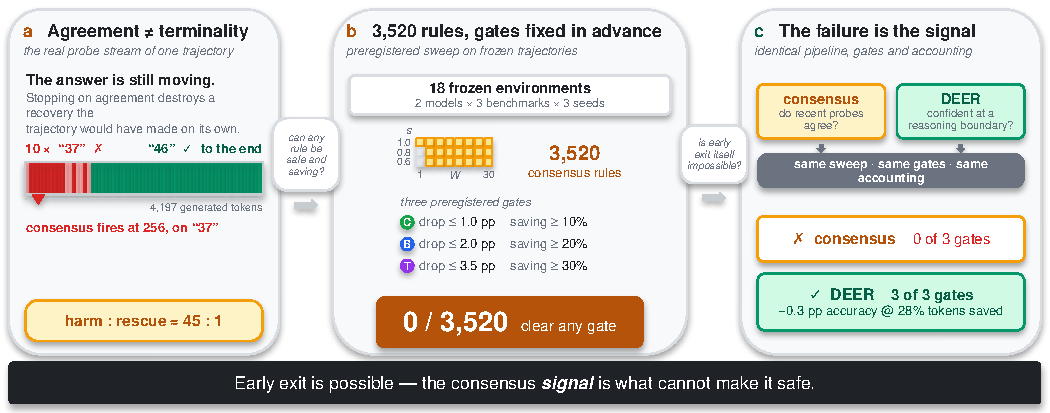
\includegraphics[width=\textwidth]{figures/gen/fig1_idea.pdf}
  \caption{\textbf{The argument in one picture.}
  \textbf{(a)} Intermediate probe agreement is not terminal. On a real
  trajectory (\textsc{MATH}500 problem~68, \dsseven{}, dense $64$-token probes)
  the model emits the same wrong answer, \texttt{37}, for ten consecutive
  probes; a rule requiring three agreeing probes fires at generated token~$256$
  and commits it. Left to run, the trajectory reaches the correct answer
  \texttt{46} and holds it for its final $47$ probes. Ribbon colours: red the
  dominant wrong answer, pink other wrong answers, green correct.
  \textbf{(b)} We ask whether \emph{any} consensus rule escapes this. A
  preregistered sweep of $3{,}520$ rules---window size $W$ $\times$ share
  threshold $s$, crossed with probe schedule, maturity, validity and
  certainty---is replayed on $18$ frozen environments against three acceptance
  gates fixed before the sweep ran. None clears any gate, and the two ways to
  fail are symmetric: capping the accuracy drop at $1$\pp{} permits $0.2\%$
  token saving, while demanding $10\%$ saving costs $2.7$\pp.
  \textbf{(c)} The failure is the \emph{signal}, not early exit. Swept through
  the identical pipeline, gates and token accounting, a boundary-confidence
  method (DEER) clears all three gates while consensus clears none---and it does
  so on the held-out test split, at $4\times$ scale and on a different
  architecture as well (Section~\ref{sec:exp-heldout}).}
  \label{fig:idea}
\end{figure*}

% ===================================================================== §4.1 ==
\begin{figure}[t]
  \centering
  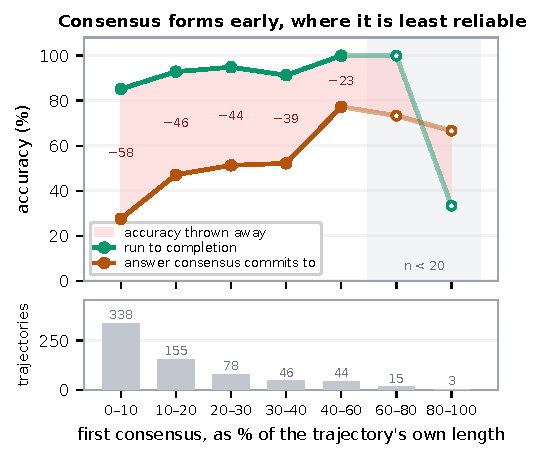
\includegraphics[width=\columnwidth]{figures/gen/fig_consensus_pos.pdf}
  \caption{\textbf{Consensus forms early, where it is least reliable.} For each
  dev-split trajectory we take the first window of three agreeing non-empty
  probes and ask two things: is that answer correct, and would the same problem
  have been correct if left to run? Position is expressed as a fraction of the
  trajectory's \emph{own} length, which controls for problem difficulty---$500$
  tokens into a $600$-token trajectory is late, $500$ into a $16$K one is not.
  Consensus forms in $679$ of $684$ trajectories, half of them within the first
  tenth, and there the committed answer is correct only $27.5\%$ of the time
  against $85.2\%$ for the same problems run to completion. The shaded gap is
  the accuracy a stop at that moment throws away. Open markers mark bins with
  fewer than $20$ trajectories; the final bin ($n{=}3$) should not be read.}
  \label{fig:consensus-pos}
\end{figure}

% ===================================================================== §4.2 ==
\begin{figure*}[t]
  \centering
  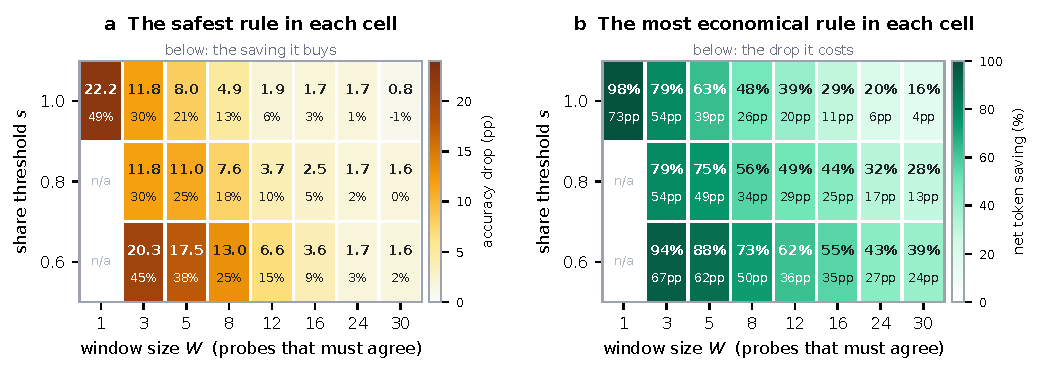
\includegraphics[width=\textwidth]{figures/gen/fig_ws_heatmap.pdf}
  \caption{\textbf{The safe-and-saving corner is empty across the entire rule
  space.} Dev split, macro-averaged over the $18$ environments. Each cell holds
  the $160$ rules that share its $(W,s)$ and differ only in the operational
  knobs, summarised by the two members a gate interrogates.
  \textbf{(a)} the cell's \emph{safest} rule: colour is its accuracy drop, and
  the number beneath is the saving that rule buys. Widening the window and
  raising the threshold does drive the drop towards the $1.0$\pp{} cap---but the
  saving falls with it, reaching $-1\%$ at $W{=}30$, $s{=}1.0$.
  \textbf{(b)} the cell's \emph{most economical} rule: colour is its net saving,
  and the number beneath is the drop it costs. Real saving is available
  everywhere, at $4$--$73$\pp. A cell would be outlined in green if any of its
  rules cleared the conservative gate (drop $\leq 1.0$\pp{} \emph{and} saving
  $\geq 10\%$); none is. The two panels are the same trade-off read from its
  two ends.}
  \label{fig:ws-heatmap}
\end{figure*}

% ===================================================================== §4.5 ==
\begin{figure*}[t]
  \centering
  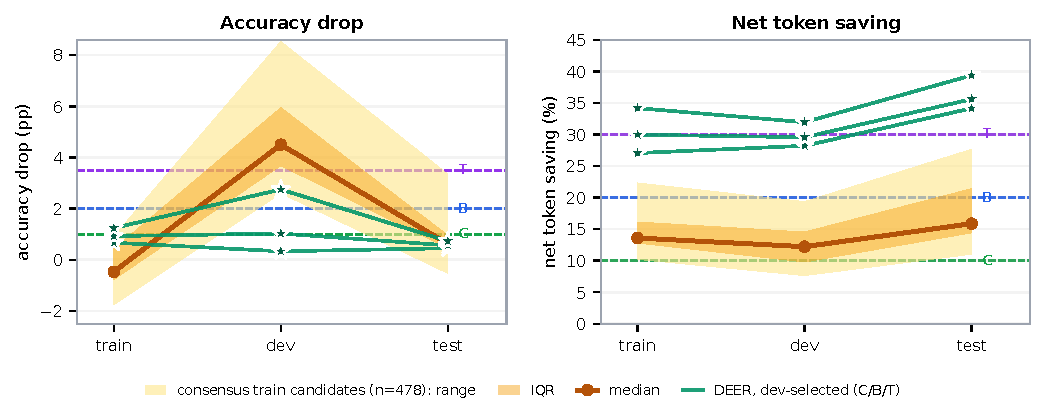
\includegraphics[width=\textwidth]{figures/gen/fig_split_transfer.pdf}
  \caption{\textbf{A rule must clear the gate on every split.} The $478$ amber
  rules are exactly those that clear the conservative gate \emph{in-sample on
  train}; drawing all $478$ would be unreadable, so we show their median,
  interquartile range and full range. Dashed lines mark all three preregistered
  gates (\textbf{C}onservative, \textbf{B}alanced, \textbf{T}oken-efficient);
  a rule must sit below them on the left and above them on the right. On dev,
  the split the gate is actually applied on, none of the $478$ does. Some
  recover on test, but a rule selected on dev is never among them: jointly,
  $0$ of $478$ clear all three splits, against $3$ of $3$ for the DEER operating
  points selected on dev. All values are macro-averaged over $18$ environments
  per split; train and dev share seeds $42$--$44$ and differ only in problems,
  while test uses unseen problems and seeds $45$--$47$.}
  \label{fig:split-transfer}
\end{figure*}

% ===================================================================== §5.1 ==
\begin{figure}[t]
  \centering
  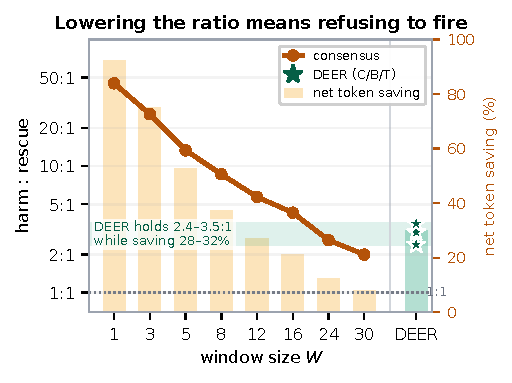
\includegraphics[width=\columnwidth]{figures/gen/fig_harm_rescue.pdf}
  \caption{\textbf{Lowering the ratio means refusing to fire.} Among stops whose
  committed answer differs in correctness from the trajectory's frozen final
  answer, we count recoveries destroyed against wrong answers banked. Pure
  sampling noise predicts $1{:}1$; a real ``continued reasoning corrects''
  effect predicts $\gg 1$. Widening the window does bring the ratio down, from
  $45{:}1$ at a latest-probe stop to $2{:}1$ at $W{=}30$---but only by stopping
  on ever fewer problems ($668 \rightarrow 121$ of $684$), so net saving
  collapses from $92\%$ to $8\%$ alongside it. DEER holds $2.4$--$3.5{:}1$
  \emph{while} saving $28$--$32\%$, which no window does. Dev split, $18$
  environments; one consensus rule per $W$ (share threshold $1.0$, probe
  interval $128$, maturity floor $512$, schema validity), with $W$ the only
  axis that varies.}
  \label{fig:harm-rescue}
\end{figure}

% ===================================================================== §5 ====
\begin{figure}[t]
  \centering
  
\includegraphics[width=\columnwidth]{figures/gen/fig_taxonomy.pdf}
  \caption{\textbf{What consensus actually stops on.} All $134$ stopped-but-wrong
  cases, labelled independently by two annotators ($\kappa = 0.82$). Only one
  case in five is one where the model had genuinely \emph{settled} on a wrong
  value; three in five are answers it had not converged on at all---a guess or
  placeholder that the probe compelled it to emit---and a further one in six are
  artifacts of the probe's output format, such as a bare option letter on a
  problem that has no options. This is the mechanism behind the accuracy tax:
  periodic probing does not read the model's belief, it \emph{forces} an answer,
  and a forced answer repeated is what a consensus rule mistakes for confidence.
  The cases were collected under a \emph{short} window (three consecutive
  agreeing certain probes, five-probe unanimity), which is precisely the regime
  in which unconverged answers dominate---consistent with the window sweep of
  Figure~\ref{fig:harm-rescue}, where enlarging the window buys accuracy back
  only by declining to fire.}
  \label{fig:taxonomy}
\end{figure}
